% !TeX program = pdflatex
% =========================================================================
%  Seminar paper -- Computer based sound production, 2026/27
%
%  Based on the official IEEE conference template (template version
%  6/27/2024, IEEEtran.cls v1.8b) from SeminarWorkTemplates26-27,
%  on A4 paper like conference-template-a4.docx.
%
%  Build:   latexmk -pdf main.tex
%           (or: pdflatex main, bibtex main, pdflatex main, pdflatex main)
%  Words:   python wordcount.py
%
%  Requirements (from the course instructions):
%    * Paper: 1400 words +/- 5 %  ->  1330 ... 1470 words
%    * Appendix - Critical Observations: 300 words +/- 5 %  ->  285 ... 315
%      (in addition to the 1400 words)
%    * At least three references from ACM, IEEE, Springer, Elsevier,
%      Elektrotehniski vestnik or Informatica
%    * Structure: introduction -> overview of the references -> your
%      contribution -> conclusions -> Appendix - Critical Observations
%      -> references
%
%  Writing style: no long dashes, colons or semicolons in the running
%  text. Every number in the text comes from ../experiment/results/.
% =========================================================================
\documentclass[conference,a4paper]{IEEEtran}

\usepackage{cite}
\usepackage{amsmath,amssymb,amsfonts}
\usepackage{graphicx}
\usepackage{textcomp}
\usepackage{xcolor}
\usepackage{url}
\usepackage{booktabs}

% Figures are taken directly from the experiment, so re-running the
% Python scripts updates the paper as well.
\graphicspath{{../experiment/figures/}}

% Placeholder: shown in red in the PDF (none left in the final text).
\newcommand{\fillin}[1]{\textcolor{red}{[#1]}}

% Notation used in several sections
\newcommand{\fs}{f_\mathrm{s}}
\newcommand{\fo}{f_0}

\begin{document}

% ---- Title --------------------------------------------------------------
% No symbols, special characters, footnotes or math in the title (IEEE).
\title{An Experimental Comparison of Antialiasing Methods for Digital
Sawtooth Oscillators}

% ---- Author -------------------------------------------------------------
\author{\IEEEauthorblockN{Urban Gaj\v{s}ek}
\IEEEauthorblockA{\textit{Faculty of Computer and Information Science} \\
\textit{University of Ljubljana}\\
Ljubljana, Slovenia \\
ug68213@student.uni-lj.si}
}

\maketitle

% ---- Abstract and keywords ------------------------------------------------
% =========================================================================
%  Abstract and keywords (IEEE: no math, symbols or citations)
% =========================================================================
\begin{abstract}
The sawtooth wave of synthesizers contains more high
frequencies than a digital signal can hold. When software computes it
sample by sample, the excess folds back as unwanted tones
called aliasing. This paper reviews three families
of antialiasing oscillators and compares a naive sawtooth, the polynomial
bandlimited step (PolyBLEP) and the second-order differentiated parabolic
waveform (DPW-2) with an ideal reference. PolyBLEP lowers the
aliasing by a median of 18 dB and DPW-2 by 11 dB, at about 1.3 to 1.5
times the cost of the naive oscillator. Two musical examples show that
aliasing matters most in high melodies.
\end{abstract}

\begin{IEEEkeywords}
aliasing, sound synthesis, oscillators, PolyBLEP
\end{IEEEkeywords}


% ---- Body (counts towards the 1400 words) --------------------------------
% =========================================================================
%  I. Introduction
% =========================================================================
\section{Introduction}

Most classic analog synthesizers create sound with subtractive synthesis.
An oscillator produces a waveform that is rich in overtones, and a filter
removes part of them to shape the timbre \cite{valimaki2007antialiasing}.
The most common starting waveform is the sawtooth, which rises in a
straight line and then drops back at once, and software synthesizers
have to compute it digitally.

A digital signal is a sequence of samples taken at a sampling rate $\fs$,
here 44.1 kHz, and it can only represent frequencies up to half of it,
the Nyquist frequency. A tone with the fundamental frequency $\fo$
consists of harmonics at $\fo$, $2\fo$, $3\fo$ and so on. Because the
sawtooth jumps once per period, its harmonics never end, and their
amplitudes fall only as $1/k$. When the waveform is sampled directly,
every harmonic above the Nyquist frequency folds back into the audible
range. A harmonic at 30 kHz, for example, appears at
14.1 kHz. These aliases do not belong to the harmonic series of the note,
so they sound like noise or out-of-tune tones. An analog recording removes them with a filter before
sampling, but a digital oscillator creates the samples directly, so
aliasing has to be prevented during generation.

Section~\ref{sec:overview} reviews three IEEE journal articles on this
problem, Section~\ref{sec:contribution} compares two cheap methods with a
naive and an ideal oscillator, and Section~\ref{sec:conclusions}
concludes.

% =========================================================================
%  II. Overview of the topic, based on the three references
% =========================================================================
\section{Overview of Antialiasing Oscillators}\label{sec:overview}

V\"alim\"aki and Huovilainen \cite{valimaki2007antialiasing} sort
antialiasing oscillators into three groups.

\subsection{Bandlimited Methods}
Additive synthesis builds the sawtooth as a sum of sine waves, one for
each harmonic, and stops at the Nyquist frequency. This avoids
aliasing, but a bass note at 55 Hz already needs 400 sine waves.
Wavetable synthesis reads precomputed bandlimited periods instead, which
becomes difficult when the pitch varies over a wide range
\cite{nam2010efficient}.

\subsection{Quasi-Bandlimited Methods}
All aliasing comes from the jump. The bandlimited impulse train (BLIT) and
the bandlimited step (BLEP) therefore replace each ideal jump with a
smoothed version whose spectrum is limited, usually read from a table
\cite{valimaki2007antialiasing}. The same article introduces PolyBLEP,
which approximates the difference between the smoothed and the ideal step
with a short polynomial. It changes only the two samples next to each
jump and needs no table.

Nam et al.\ \cite{nam2010efficient} build each pulse of a BLIT from a
low-order fractional delay filter, a short filter that can place an
impulse between two samples, and judge the remaining aliases with models
of human hearing. With a third-order
B-spline filter, the waveforms were perceptually free of aliasing up to a
fundamental frequency of 5.8 kHz.

\subsection{Alias-Suppressing Methods}
The differentiated polynomial waveform (DPW) uses the fact that smoother
waveforms have weaker high harmonics. Its second-order form, DPW-2,
squares the naive sawtooth into a parabola. The parabola has no jump and
its harmonics fall as $1/k^2$, so much less energy folds back. The
difference of neighbouring samples then turns it back into a sawtooth.
V\"alim\"aki et al.\ \cite{valimaki2010dpw} extend this idea to higher
orders and found the fourth-order version perceptually free of aliasing
over the whole range of a grand piano. Nam et al.\
\cite{nam2010efficient} found, however, that by their hearing model low
orders alias audibly already at relatively low pitches.

% =========================================================================
%  III. Contribution: experimental comparison
%  Numbers come from ../experiment/results/summary.json, cpu.csv and
%  demo_aliasing.csv. Figures 1 and 2 are made by paper_figures.py, the
%  others by run_experiment.py.
% =========================================================================
\section{Experimental Comparison}\label{sec:contribution}

Four oscillators were implemented in Python with NumPy. The code, data
and audio files are submitted with this paper.

% -------------------------------------------------------------------------
\subsection{Oscillators}\label{sec:oscillators}
All four use a phase $\varphi[n]$ that grows by $T = \fo/\fs$ every
sample and wraps from 1 back to 0. The naive oscillator turns it directly
into a sawtooth,
\begin{equation}
  s[n] = 2\varphi[n] - 1, \qquad
  \varphi[n] = \left(n\,\fo/\fs\right) \bmod 1 .
  \label{eq:naive}
\end{equation}
PolyBLEP computes $y[n] = s[n] - r[n]$, where the correction $r$ is
non-zero only in the samples just after and just before each jump
\cite{valimaki2007antialiasing},
\begin{equation}
  r[n] =
  \begin{cases}
    2t - t^2 - 1, & t = \varphi[n]/T, \quad \varphi[n] < T,\\
    t^2 + 2t + 1, & t = (\varphi[n]-1)/T, \quad \varphi[n] > 1-T,\\
    0,            & \text{otherwise}.
  \end{cases}
  \label{eq:polyblep}
\end{equation}
DPW-2 squares the naive sawtooth and takes the difference of neighbouring
samples \cite{valimaki2010dpw},
\begin{equation}
  y[n] = \frac{s^2[n] - s^2[n-1]}{4T},
  \label{eq:dpw}
\end{equation}
where the division by $4T$ restores the amplitude. The additive reference
sums only the harmonics below the Nyquist frequency,
\begin{equation}
  y[n] = -\frac{2}{\pi}\sum_{k=1}^{K}\frac{\sin(2\pi k\varphi[n])}{k},
  \qquad K = \left\lfloor \frac{\fs}{2\fo} \right\rfloor .
  \label{eq:additive}
\end{equation}

Fig.~\ref{fig:waveforms} shows why the naive oscillator fails. Its samples
lie exactly on the analog waveform, whose jump contains infinitely high
frequencies. PolyBLEP and DPW-2 move the samples next to the jump towards
those of the ideal additive signal.

\begin{figure}[!t]
  \centering
  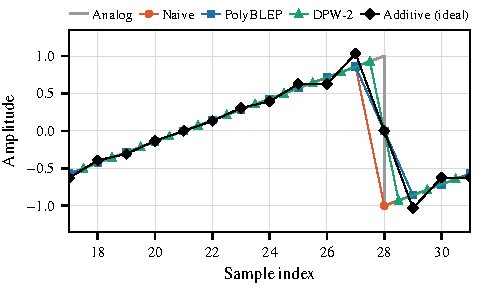
\includegraphics[width=\columnwidth]{fig_waveforms}
  \caption{Samples around one jump of a 3.15\,kHz sawtooth. DPW-2 is
  shifted by half a sample to remove its delay.}
  \label{fig:waveforms}
\end{figure}

% -------------------------------------------------------------------------
\subsection{Measuring Aliasing}\label{sec:method}
Aliasing was measured with the alias-to-harmonic ratio,
\begin{equation}
  \mathrm{AHR} = 10\log_{10}
  \frac{\sum_{f \in \mathcal{A}} |X(f)|^2}{\sum_{f \in \mathcal{H}} |X(f)|^2}
  \ \mathrm{dB},
  \label{eq:ahr}
\end{equation}
where $X(f)$ is the spectrum, $\mathcal{H}$ the frequencies within 2.7 Hz
of a harmonic and $\mathcal{A}$ all other frequencies between 20 Hz and
20 kHz. An AHR of $-30$ dB means that the aliases carry one thousandth of
the harmonic power. Fig.~\ref{fig:spectra} shows the spectra of one note,
where every line without a circle is an alias.

\begin{figure}[!t]
  \centering
  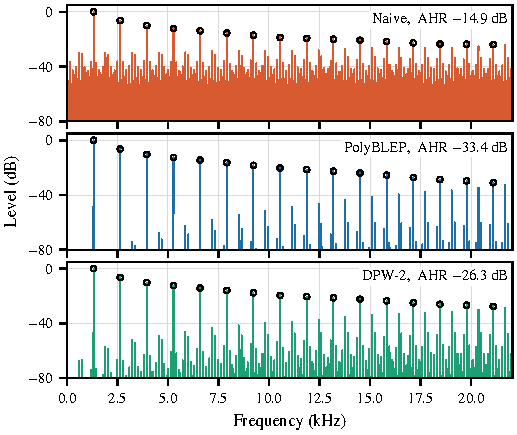
\includegraphics[width=\columnwidth]{fig_line_spectra}
  \caption{Spectra of the note E6 (1319\,Hz). Circles mark the
  harmonics.}
  \label{fig:spectra}
\end{figure}

\begin{figure}[!t]
  \centering
  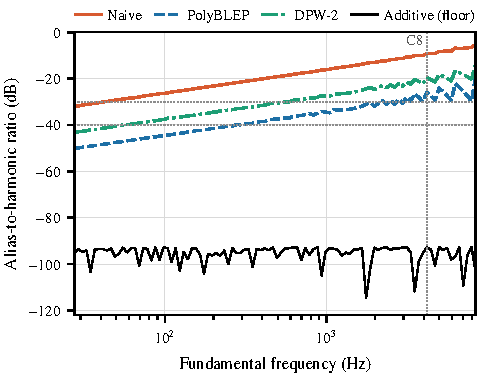
\includegraphics[width=\columnwidth]{fig_ahr}
  \caption{AHR for every note from A0 to C9. Dotted lines mark $-30$\,dB,
  $-40$\,dB and C8.}
  \label{fig:ahr}
\end{figure}

\begin{figure*}[!t]
  \centering
  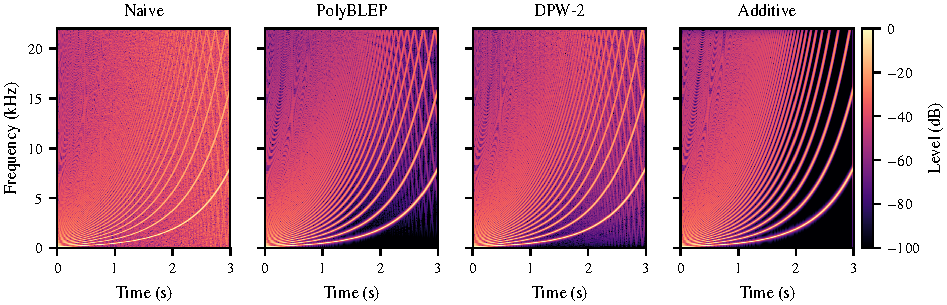
\includegraphics[width=\textwidth]{fig_spectrograms}
  \caption{Spectrograms of a 3\,s sweep from 100\,Hz to 8\,kHz. Rising
  lines are harmonics and the rest are aliases.}
  \label{fig:spectrograms}
\end{figure*}

The AHR was computed from a $2^{17}$-point FFT with a Blackman-Harris
window for all 100 notes from A0 (27.5 Hz) to C9 (8.4 kHz). For 17 notes,
such as G1, G2 and G3, the aliases land almost exactly on harmonics and
would be counted as harmonic power, so these notes were raised by up to
six cents, a few hundredths of a semitone. The AHR was also computed
with A-weighting, which weights each frequency by the sensitivity of the
ear. Finally, the harmonics of a 440 Hz tone were compared with the ideal
amplitudes $2/(\pi k)$, and computation times were measured.

% -------------------------------------------------------------------------
\subsection{Results}\label{sec:results}
Fig.~\ref{fig:ahr} and Table~\ref{tab:summary} show that the additive
oscillator stays between $-115$ and $-93$ dB, the noise floor of the
analysis. For the others, aliasing grows with pitch,
because a higher note has more of its energy above the Nyquist frequency.
The naive oscillator exceeds $-30$ dB for every note above E1 (41 Hz) and
reaches $-9$ dB at C8, the top note of the piano. PolyBLEP lowers the AHR
by 14 to 23 dB, with a median of 18 dB, and stays below $-30$ dB up to
C7 (2.1 kHz). DPW-2 lowers it by 9 to 14 dB, with a median of 11 dB, and
stays below $-30$ dB up to C\#5 (554 Hz).
A-weighting makes the corrected oscillators look better at high notes,
because their remaining aliases lie near the Nyquist frequency, where the
ear is less sensitive.

\begin{table}[!t]
  \caption{AHR in dB at Selected Notes, Highest Note Below $-30$\,dB and
  Time Relative to Naive at 440\,Hz}
  \label{tab:summary}
  \centering
  \setlength{\tabcolsep}{4pt}
  \begin{tabular}{lrrrrcr}
    \toprule
    Method & A2 & A4 & A6 & C8 & Limit & Time \\
    \midrule
    Naive    & $-25.8$ & $-19.7$ & $-13.4$ & $-9.3$  & E1   & 1.00 \\
    PolyBLEP & $-44.1$ & $-37.8$ & $-31.1$ & $-25.8$ & C7   & 1.32 \\
    DPW-2    & $-37.0$ & $-30.9$ & $-24.4$ & $-19.6$ & C\#5 & 1.45 \\
    Additive & $<-92$  & $<-92$  & $<-92$  & $<-92$  & all  & 14.4 \\
    \bottomrule
  \end{tabular}
\end{table}

The spectrograms of a rising sweep in Fig.~\ref{fig:spectrograms} show the
same order. The naive sweep is covered with aliases from
the start, PolyBLEP leaves only weak ones, and DPW-2 lies in between.

Both corrections also make the wanted high harmonics slightly quieter
(Fig.~\ref{fig:harmonics}). For a 440 Hz tone, PolyBLEP lowers the
harmonic at 19.8 kHz by 6.2 dB and DPW-2 by 3.1 dB, so DPW-2 keeps more
brightness but aliases more.

\begin{figure}[!t]
  \centering
  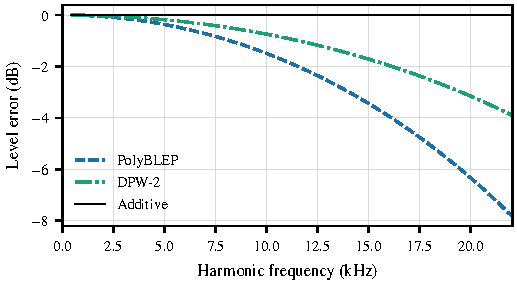
\includegraphics[width=\columnwidth]{fig_harmonics}
  \caption{Level error of the harmonics of a 440\,Hz tone.}
  \label{fig:harmonics}
\end{figure}

At 110, 440 and 1760 Hz, PolyBLEP and DPW-2 take 1.29 to 1.45 times as
long as the naive oscillator. Additive synthesis is 52 times slower at
110 Hz and 4.7 times at 1760 Hz, because lower notes need more sine
waves. These NumPy timings show relative cost only.

Two short clips show what this means in music (Table~\ref{tab:demos}).
Each was rendered with all four oscillators. In a bright lead melody
between E5 and C7 with vibrato, the aliases of the naive oscillator are
only 15 dB below the music, and PolyBLEP lowers them to $-33$ dB. In a
bass line around A1 played through a lowpass filter, the filter removes
the high aliases of PolyBLEP, which reaches $-73$ dB. The naive oscillator
also aliases far below the cutoff, so it only reaches $-33$ dB, close to
the $-29$ dB of an unfiltered A1. A filter therefore cannot replace an
antialiasing oscillator.

\begin{table}[!t]
  \caption{Aliasing in the Musical Examples in dB}
  \label{tab:demos}
  \centering
  \begin{tabular}{lrrr}
    \toprule
    Clip & Naive & PolyBLEP & DPW-2 \\
    \midrule
    Lead melody & $-15.0$ & $-33.3$ & $-26.4$ \\
    Bass line   & $-32.6$ & $-72.6$ & $-51.1$ \\
    \bottomrule
  \end{tabular}
\end{table}

% -------------------------------------------------------------------------
\subsection{Limitations}\label{sec:discussion}
The AHR ignores masking, the effect that a loud sound hides quieter sounds
nearby, so the thresholds are illustrations rather than
limits of audibility. Only DPW-2 was tested, although higher orders
perform better \cite{valimaki2010dpw}, and no formal listening test was
carried out.

% =========================================================================
%  IV. Conclusions
% =========================================================================
\section{Conclusions}\label{sec:conclusions}

A naive sawtooth aliases over the whole musical range, and more so at
higher pitch. PolyBLEP corrects only two samples per jump, yet it removes
about 18 dB of aliasing at roughly 1.3 times the cost and keeps the AHR
below $-30$ dB up to C7. DPW-2 is about as cheap and keeps more of the
high harmonics, but its median improvement of 11 dB agrees with the
observation in \cite{nam2010efficient} that low-order DPW aliases already
at moderate pitch. The musical examples show that aliasing matters most
in high melodies.

For a simple software synthesizer, PolyBLEP is therefore a sensible
default. Higher-order DPW or BLIT with fractional delay filters
\cite{valimaki2010dpw,nam2010efficient} are needed when aliasing must stay
inaudible across the whole keyboard. A listening test would be a natural
next step.


% ---- Appendix (counted separately: 300 words) ----------------------------
%TC:ignore
% =========================================================================
%  Appendix - Critical Observations
%  Required: 300 words +/- 5 %  (285 ... 315), NOT part of the 1400 words.
%  Placed after the Conclusions and before the References (as required).
%
%  Evaluate critically the session with the LLM you used for this seminar:
%  mistakes, hallucinations, incomplete information, ... The complete
%  session (as PDF) is uploaded to Moodle together with the paper.
%
%  DRAFT written from the documented events below and from the session
%  of 24-25 Nov 2026 (musical examples, paper merge). Check every
%  statement against your session PDFs and change it to your own view.
%
%  Things from the session you may want to look at (check them against
%  the session PDF yourself; your own assessment is what counts):
%   - Literature: venues and page numbers were checked with web search,
%     but the paper summaries were based on the full text for only one
%     of the three papers (abstracts and index records for the others),
%     which the LLM stated itself.
%   - The explanation of additive synthesis used a Fourier series with a
%     different phase (sign pattern (-1)^(k+1)) than the code, where the
%     series is aligned with the naive sawtooth.
%   - The first draft of the comparison code had two measurement errors
%     that the LLM found only when testing it: fundamental frequencies
%     at which aliases fell onto harmonics (a false 81 dB result), and
%     float32 phase accumulation drift that made even the additive
%     reference look bad.
%   - When merging the code it found a real error in your own
%     measurements (aliases hidden in the guard band at G1, G2, G3,
%     which inflated the maximum improvement figures).
%   - Claims stated as expectations without proof (e.g. how PolyBLEP
%     and DPW-2 relate) vs. claims backed by measurement.
%   - Numbers the LLM reported from its own environment (e.g. timings)
%     vs. numbers you reproduced.
%   - Session of 24 Nov: the first aliasing measure for the musical
%     examples counted the treble loss of PolyBLEP/DPW-2 as aliasing and
%     ranked DPW-2 above PolyBLEP; corrected after comparing with the AHR.
%     Code estimate 100-150 lines, final demo.py 293 lines.
%   - The old paper draft quoted additive cost 190x/41x/7.9x, the current
%     data says 52x/14x/4.7x (code was optimised after the text).
% =========================================================================
\section*{Appendix - Critical Observations}

Throughout this seminar I used a large language model, Claude, for the
literature search, the Python experiment, the musical examples and the
text. It saved a lot of time, but almost every part needed checking.

The bibliographic details were reliable, because the model verified
venues, volumes and page numbers with web search. Its summaries, however,
were based on the full text of only one of the three articles and on
abstracts for the other two, which it stated itself. The specific claims
in the overview therefore had to be checked against the sources before
they could be used.

The code contained errors that the model found only when it tested its
own work. The first measurement reported a false result of 81 dB at notes
where aliases fell exactly onto harmonics, and phase accumulation in
single precision made even the ideal reference look bad. Later it found a
similar error in my own measurements, where aliases hidden next to
harmonics at G1, G2 and G3 inflated the best results. For the musical
examples, its first measure counted the intended treble loss of PolyBLEP
and DPW-2 as aliasing and ranked DPW-2 above PolyBLEP. The model noticed
this only because the ranking contradicted the main experiment, and then
corrected it.

Other problems were inconsistencies rather than errors. The explanation of
additive synthesis used a Fourier series with a different sign pattern
than the code. An earlier draft of the paper still quoted the cost of
additive synthesis from before the code was optimised. The model also estimated the code for the musical
examples at about half of its final length.

Overall, the model was most trustworthy when it checked its claims
against measured data. It was least trustworthy when it summarised
sources it had not fully read or stated expectations before measuring
them.

%TC:endignore

% ---- References ------------------------------------------------------------
% Entries are in refs.bib; only the ones you \cite appear in the list.
%TC:ignore
\bibliographystyle{IEEEtran}
\bibliography{refs}
%TC:endignore

\end{document}
